%%------------------------------------------------------
%  
%  Implementation include for dissertation
%
%------------------------------------------------------

Implementing Partridge from a set of initial designs proved to be a
challenging but rewarding process. There were a great number of technical
challenges involved in building the system, a large proportion of the
implementation time was spent working on the paper preprocessor module.
However, some aspects of the web interface and backend were also quite
difficult to tackle. 

\section{Paper Preprocessor}

Partridge's Paper Preprocessor module was the most difficult part of the
project to implement. From acquiring papers for use in the project to teaching
a machine learning system to recognise different types of scientific
publication, a number of technical challenges were encountered.

\subsection{ Sourcing and Acquiring Scientific Papers}

In order to provide a useful service to researchers looking for papers, growing
a large corpus of scientific literature was made a high priority during the
project. This was especially important when training the Machine Learning
models since training data sets need to be statistically significant in order
to provide any meaninful results. Users are given the option, and actively
encouraged, to upload papers that they own or publish on another author's
behalf to the Partridge instance. However, to speed up this process, a number
of papers were acquired from various open access sources.

The most convenient and accessible source was the ART corpus that SAPIENTA was
trained with\cite{citeulike:11077287}. This corpus was already stored using the
CoreSC schema and had been pre-annotated. This meant that Partridge would not
need to do any conversion or pre-processing on the papers. The papers in this
corpus were all of a similar type and covered similar subject areas within the
domain of Biochemistry. There were also approximately 260 papers in the
collection. These papers were used to help establish a conversion process from
PDF to annotated XML. However, they only formed part of the final corpus.
Including a large number of papers from other sources provided a more
comprehensive collection of data for Partridge to learn from.

The `mega-journals' PLOSOne \url{http://www.plosone.org/} and arXiv
\url{http://www.arxiv.org/} were suggested as sources for more open access
articles that could be added to Partridge. Both of these sites were found to
contain large volumes of open access papers. Most of the articles stored on the
arXiv site were in PDF format which, as discussed below, are difficult to
convert and annotate. However, PLOSOne use the SciXML markup language for
papers published through their journal, which made converting and annotating
them a lot simpler for Patridge. PLOSOne also publish all of their papers under
the Creative Commons Share-Alike-By-Attribution license\cite{ccbyattr}. This
meant that as long as the author information was left intact, all of the papers
could be used for data mining purposes.

A third mega-journal used for downloading papers was the PubMed Centrala (PMC)
repository \url{http://www.ncbi.nlm.nih.gov/pmc/}. Not all of
the papers available for viewing at the PMC website are open access. However,
they do offer a listing for the subset of open access papers available on their
website. The PubMed Central format is also very similar to the SciXML format
and compatible with SAPIENTA. Therefore, a large number of PubMed papers were
also used for the initial training of Partridge.

\subsection{Format Conversion} Most scientific papers available on the internet
are formatted as PDF documents. However, Partridge uses and stores documents as
XML markup and uses the CoreSC schema by Soldatova and
Liakata\cite{liakata2008guidelines} for annotation. Therefore some spike work
was carried out to determine the feasibility of converting papers published as
PDF documents into XML documents. Townsend \emph{et al.} (2009) liken
converting PDF to XML to ``converting hamburgers into cows," they go on to
explain that PDF documents do not contain any semantic data and documents lose
much of their explicit structure when they are formatted in this way
\cite{Townsend2009}.  Therefore, to convert PDF documents into an NLP-friendly
format, some heuristics must be used to detect the document's
structure\cite{pdfminer}.

This was the first big challenge in the project. A prototype script was written
using a Python PDF extraction library called PDFMiner
(\url{http://www.unixuser.org/~euske/python/pdfminer/index.html}).  This
toolkit already contains some heuristics about how to extract text from PDF
documents, grouping together characters that appear very close to each other,
and separating paragraphs and headings when a larger area of whitespace is
detected\cite{pdfminer}. Despite these rules, the library still produced some
extraneous whitespace and newline characters as part of the output. A
subroutine to trim whitespace and newlines was added to the script to resolve
this problem. 

The next stage was to split the text into sentences in preparation for
processing with SAPIENTA. With the assistance of the NLTK library, a sentence
splitting subroutine was implemented. This used a machine learning algorithm
that had been trained to recognise sentence boundaries to split the text. Each
sentence was then added to a CoreSC compatible XML document for processing by
SAPIENTA.

Initially, the PDF conversion subroutine had a very high error rate due to the
variation in the formatting of scientific papers. It was suggested that PDFX
(\url{http://pdfx.cs.man.ac.uk/}), a free service hosted by the University of
Manchester could be used instead of PDFMiner for the initial PDF data
extraction. The main advantage of PDFX over the PDFMiner library is that it is a
trained machine learning system that has been trained using a large full-text
selection of scientific articles; PDFMiner uses more general heuristics
designed to process a large selection of different types of PDF document.

PDFX also provides output that already has some metadata, such as title,
author, and abstract, associated with it. PDFMiner did not provide any
metadata, and it was necessary for the script to guess which passage of text
was the abstract after the initial text extraction stage.

With the new PDF extraction method in place, the script ran without the need
to modify either of the whitespace sanitiser or sentence splitter routines. The
process was much more successful and able to produce SAPIENTA-compatible
documents from most of the PDF input files that were provided.

\subsection{Annotating with SAPIENTA}

With a successful PDF conversion script, the next step was to try and run
SAPIENTA over the converted papers and annotate them, ready for inclusion in
the Partridge corpus.

By default, SAPIENTA is packaged as a web-based tool, written in Java, that
can be downloaded (from \url{http://www.sapientaproject.com/software}) and used
to annotate one paper at a time. Dr Liakata was able to provide information on
two alternative ways of using the system. One method was to submit a remote
procedure call (RPC) to a server running SAPIENTA with a batch of papers and
retrieve the output. The other method was to use an alternative version of the
code that runs locally in a Python environment and could be modified to process
papers as a batch.

A script was written to send un-annotated XML documents to the remote SAPIENTA
server and retrieve a list of annotations. This worked well until the server
stopped replying to requests. This meant that no further conversions could be
carried out until the server was repaired and raised concerns about how the
remote servers might cope with a large number of automated requests from a
full version of Partridge.

The Python version of SAPIENTA was then downloaded and a test executed.
Unfortunately there were several data files missing from the package that had
to be acquired from Dr Liakata. 

SAPIENTA for Python also relies upon a package called CRFSuite which implements
Conditional Random Fields, a method for segmenting and labelling sequence
data\cite{CRFsuite}. This library did not compile properly on the test
environment and its creator had to be contacted via a mailing list (See
Appendix \ref{sec:crfemail}). After a few days, the owner responded and the
library was compiled successfully.  

Once all the data files and libraries were successfully in place, the Python
version of SAPIENTA was used to process some of the papers converted from PDF.
This appeared to have been successful. However, after applying some machine
learning evaluation techniques as discussed in Chapter \ref{chapter:testing},
it was clear that the Python version of SAPIENTA was not accurate enough to
provide CoreSC annotations, scoring 44\% accuracy on average. After discussion
with its author, it became apparent that some of the features provided in the
server-side version of SAPIENTA had not been implemented in the Python code
yet. Therefore, it was necessary to switch bak to remote annotation.

\subsection{Paper Type Classification}

Once a large number of papers had been acquired from ART, PlosOne and PubMed
Central, work could begin on implementing a paper type classifier able to
discriminate between ``Case Study", ``Research" and ``Review" papers. However,
for a machine learning classifier to discriminate between classes of data, it
is necessary to choose a set of features that differ as much as possible
between the classes. For example, to discriminate between cats and dogs,
``number of legs" is a poor feature since both species normally have 4.
However, the noise that these animals make may be a good discriminative feature
since cats tend to mew and dogs bark. 

\subsubsection{Feature Selection and CoreSCs}

There are several well established features used for classifying text within
the NLP community. However, since Partridge has access to CoreSC annotations
for each paper, an investigation was carried out into how useful CoreSC data
can be as a feature for paper type discrimination. Every sentence in a given
annotated paper has an associated CoreSC label. It is therefore trivial to
calculate the proportion of a paper made up of sentences with a specified
CoreSC type. Several papers were manually inspected and the proportions of each
CoreSC represented within were calculated. A pattern quickly emerged between
the types of paper and the proportions of each CoreSC within them. 

\begin{figure}[!h]
\centering
\begin{subfigure}[b]{0.6\textwidth}
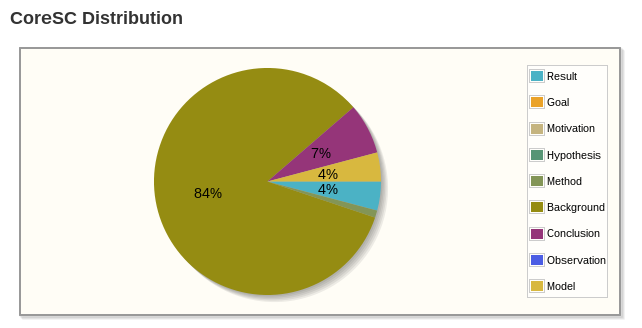
\includegraphics[width=\textwidth]{images/implementation/review_corescs.png}
\caption{CoreSC content for a sample review paper}
\end{subfigure}
\begin{subfigure}[b]{0.6\textwidth}
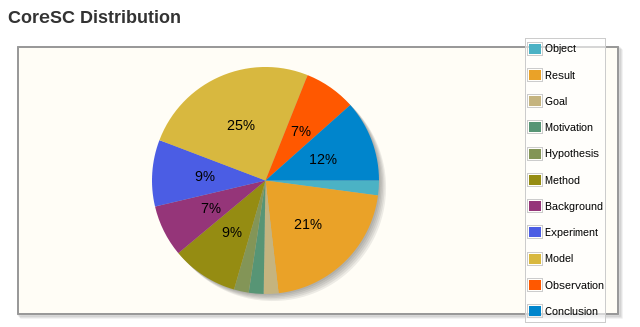
\includegraphics[width=\textwidth]{images/implementation/report_corescs.png}
\caption{CoreSC content for a sample research paper}
\end{subfigure}

\caption{Contrasting CoreSC content of Review and Research Papers}
\label{fig:coresc_pies}
\end{figure}

Figure \ref{fig:coresc_pies} shows the CoreSC content of a review paper and a
research paper randomly selected from the corpus. The review papers tend to be
made up almost entirely from Background CoreSC sentences. However, research
papers are much more evenly spread, made up of several different types of
CoreSC. This investigation suggested that there is almost certainly a discriminative
relationship between CoreSC categories and a paper's type. 

\subsubsection{ K-means clustering}

Before working with supervised learning systems, a preliminary experiment was
carried out to see whether clustering papers using the K-means algorithm could
successfully identify the paper types, thus removing the need to train and
maintain a supervised model. This was also an excellent opportunity to explore
the data and try and detect any inherent patterns within the papers.

K-means clustering uses the Euclidean distance between each data sample to
decide which cluster it is closest to and should belong to. K is the number of
clusters that are used and is decided ahead of execution. K-means clustering is
often run multiple times using a range of K values when the number of clusters
in the data is unknown. The performance of the clustering algorithm is often
evaluated using the K-means silhouette which is a measurement of how tightly
the data is clustered. A low silhouette value ($K \approx 0$) suggests loose
clustering and therefore little correlation, a high silhouette value ($K
\approx 1$) corresponds with very tight clustering and good correlation.

All of the papers were manually identified as either a ``Case Study", a
``Review Paper" or a ``Research Paper." They were then loaded into a script and
clustered using their CoreSC respective compositions. K-Means silhouettes were
used as a measure of how effective the clustering process was. This was
repeated for $ K \in [2..8] $ and the best silhouette measurement and value for
K retained. The algorithm consistently showed that K=3 was the best K value.
However, the silhouette value was consistently low. It was suggested that this
may have been because all CoreSC types were considered equally; the less
discriminative CoreSCs may have been offsetting the effect of the highly
discriminative ones.

To remedy this, all papers were again clustered, but using only three CoreSC
labels at a time: reducing the noise from the less important types. The
algorithm was run for all combinations of 3 CoreSC labels, again retaining only
the most successful combination of features and K value based upon the K
silhouette value. This returned a set of much stronger K silhouette values in
general. The algorithm also determined that the combination of ``Background",
``Motivation" and ``Method" CoreSC labels seemed to be the most
discriminative, providing a silhouette value of 0.63. 

\begin{figure}[!ht]
\centering
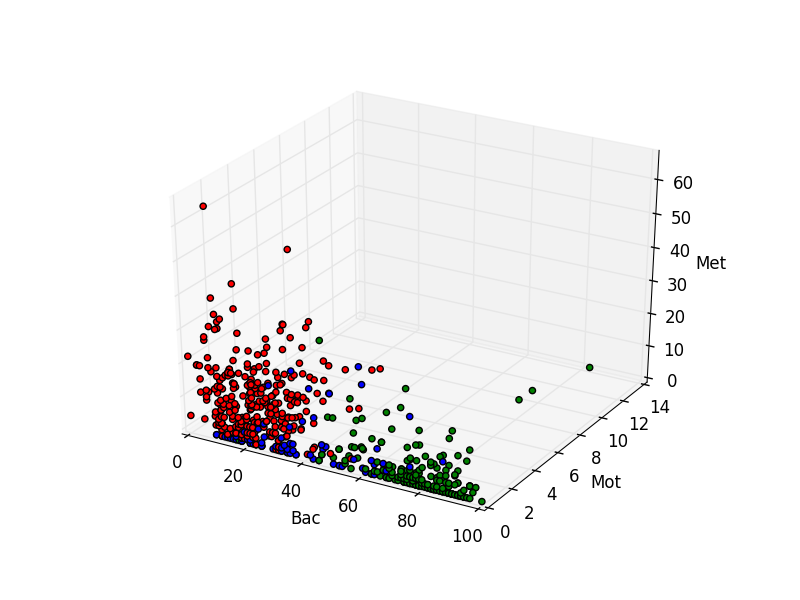
\includegraphics[width=0.8\textwidth]{implementation/cluster.png}
\caption{Paper types rendered using Bac, Met and Mot CoreSCs}
\label{fig:clusters}
\end{figure}

Figure \ref{fig:clusters} shows the papers from the corpus rendered in 3
dimensions using their Background, Method and Motivation CoreSC makeup.
Although the data does not cluster perfectly by class, these three categories
do provide fairly clear discrimination between the three types of paper. 

Clustering the papers did not seem to provide a reliable way to classify them
by type and it was decided that better results could be obtained through the
use of a supervised learning classifier instead. However, the three most
discriminative CoreSC types were chosen as features for the learner.

\subsubsection{Random Forest Learner}

To classify the papers, a Random Forest Learner was trained using a subset of
the Partridge corpus using Background, Method and Motivation CoreSC information
from the papers. The classifier was found to be highly accurate, correctly
predicting a paper's type in 87.9\% of cases. The classifier's accuracy and
evaluation are further discussed in Section \ref{sec:evaluation_learners}
below. 

The new classifier was incorporated into the paper preprocessor and triggered
after SAPIENTA annotation for each new paper. It was also called
retrospectively for papers in the Farnsworth Partridge instance that were not yet
classified.


\subsection{ Paper Processing Notifications }

Providing notifications to users when a paper has been processed was not part
of the original design for Partridge. The feature was added to the system after
being raised as a potential improvement by one of the test users. Previously,
users to added papers to the Partridge corpus did not know whether the
operation was a success unless they ran a search and the paper appeared in
their results. Adding email notifications to Partridge significantly improved
the user experience for paper uploaders. The uploader is given the option to
provide their email address when they send the paper to the Partridge server.
Once the preprocessor has converted, annotated and classified a paper, an email
is sent to the uploader informing them that the paper has been added to the
database and containing a direct link to the paper's profile page.

The system also emails users upon failure, allowing them to report the error to
the GitHub page if required and also providing closure for users who are unsure
why their paper isn't appearing in Partridge queries.



\section{ Web Backend }

The Partridge web backend was much easier to implement than the preprocessor.
The web framework Flask was used to do a lot of the hard work such as routing
requests and encoding data into browser-compatible formats.

\subsection{ Server Views }

Flask provides a model-view-controller style framework in which specific web
URLS are represented by `view' functions. The behaviour of these views changes
dependent upon data from the incoming HTTP request. Their return value is
encoded as an HTTP response and sent back to the browser that made the request.

The implementation of the server views was for the most part straight forward
with the exception of some of the responses to the interactive web elements in
the HTML markup. It was determined that the best way to communicate between
frontend and backend elements interactively was to encode responses as
JavaScript Object Notation JSON - a common notation used to describe arbitrary
data structures\cite{jsonRFC}. Despite its name, JSON encoders and decoders are available for
most common programming languages.  Flask even has an inbuilt method called
jsonify which can be used to automatically encode arbitrary Python objects as
JSON and send it back to the browser for parsing by the frontend scripts.

\subsection{Database Interaction \& SQLAlchemy}

\subsection{Data version control \& Alembic}

During the development of Partridge, the structure of the SQL database used to
store the papers changed a lot due to modifications to the ORM modules as
discussed above. These structural changes meant that the production database at
\url{http://farnsworth.papro.org.uk/} and the development database were not
compatible and that updates to the code on the development server would break
the application on the production server unless the database structure was also
updated. 

To prevent this from happening, a Python utility called
Alembic\cite{alembic2013} was used for keeping the Database structure under
Version Control. Alembic is executed when Partridge's ORM models are modified
and can detect differences in database structure between the SQLAlchemy model
in Partridge's source code and the live database. It generates sets of SQL
commands that are used to synchronise the database structure with the most
recent program structure. This allowed the Farnsworth database to be updated
automatically when a new change to Partridge's data structures was made rather
than having to be purge and repopulate it.

\subsection{WSGI and Apache Integration}

Flask provides a test server that can be used for developing your web
application. However, it is written in python and is not designed to be as
stable or scalable as a full web server application such as Apache. Once
Partridge's basic web interface was complete and the application ready to be
deployed, it had to be integrated into Apache to provide stable web server
support.

By default, Apache only serves static HTML content and image/data files. It makes
use of plugins to support dynamic web pages, in languages such as PHP and
Python. A plugin called WSGI is used to allow Apache to serve Python
applications. WSGI requires that the Python program exposes an
\emph{application} object which implements a common interface in order to
communicate with Apache.

After thorough investigation, it was discovered that Flask provides a WSGI
compatible \emph{application} object. A small wrapper was written that exposes
the Flask app to WSGI and the server began to work as expected. Unfortunately,
the WSGI interface didn't allow the preprocessor daemon to be run in the
background. Therefore, a second wrapper was created that allowed the execution
of the Paper daemon as a standalone process.

\section{Web Frontend}

\subsection{Query Interface}

\subsection{ Paper Upload Interface }

\subsection{ Bookmarklet }

One of the most important user suggestions for improving the usability of
Partridge and facilitating the rapid expansion of the paper corpus was the
Paper Upload Bookmarklet. The bookmarklet was not in the initial system design
and was added as an extra feature towards the end of the project. It allows
users browsing sites such as PubMed Central and PlosOne to add papers that
interest them to Partridge without having to download the paper from the
journal and upload it to the Partridge server manually. 

The system is implemented as a standard web page wrapped inside a javascript
bootstrap module that can be added as a bookmark to a user's web browser. When
the user finds a paper that they wish to add to Partridge on one of the
compatible journal sites, they click the bookmark, loading an embedded frame in
their current browser window and automatically uploading the paper that the
user is looking at to Partridge's server. 

The bookmarklet trivialises the act of adding new papers to Partridge and this
should help to encourage users to help grow Partridge's paper corpus. 
